% ---------------------------------------------------------------------------
%  CSEDU 2027 submission -- double-blind review version.
%  Built on the SCITEPRESS conference template (SCITEPRESS.sty, apalike).
%  Compile:  pdflatex paper && bibtex paper && pdflatex paper && pdflatex paper
% ---------------------------------------------------------------------------
\documentclass[a4paper,twoside]{article}

\usepackage{epsfig}
\usepackage{subcaption}
\usepackage{calc}
\usepackage{amssymb}
\usepackage{amstext}
\usepackage{amsmath}
\usepackage{amsthm}
\usepackage{multicol}
\usepackage{pslatex}
\usepackage{apalike}
\usepackage{algorithm2e}
\usepackage[bottom]{footmisc}
\usepackage{graphicx}
\PassOptionsToPackage{hyphens}{url}
\usepackage{url}
\usepackage{booktabs}
\usepackage{array}
\usepackage{tikz}
\usetikzlibrary{arrows.meta, positioning, calc}
\usepackage[utf8]{inputenc}
\usepackage[T1]{fontenc}
\usepackage{SCITEPRESS}     % Please add other packages that you may need BEFORE the SCITEPRESS.sty package.


% Textual citation for apalike labels: "Author et al. (Year)" instead of "(Author et al., Year)".
\makeatletter
\def\@citetsplit#1, #2\@nil{#1 (#2)}
\newcommand{\citet}[1]{\if@filesw\immediate\write\@auxout{\string\citation{#1}}\fi
  \@ifundefined{b@#1}{{\bfseries ?}}{\expandafter\expandafter\expandafter\@citetsplit\csname b@#1\endcsname\@nil}}
\makeatother

% Short-hand for process-state names
\newcommand{\st}[1]{\textsc{#1}}

\begin{document}

\title{A Hybrid Graph-Table Interface for Study Planning: Design and an Observational Study of How Students Plan with It}

% ---- Double-blind review version: author block left anonymous. ----
% ---- For the camera-ready version, restore the \author block from the ----
% ---- template (Example.tex) with names, affiliations, e-mails and ORCIDs. ----
\author{\authorname{Anonymous Author(s)}
\affiliation{Anonymous Affiliation}
\email{anonymous@example.org}
}

\keywords{Study Planning, Curriculum Visualisation, Educational Dashboards, Educational Recommender Systems, User Study, Higher Education.}

\abstract{Students plan their studies against curricula that encode prerequisites, electives and institutional rules, and the tools that support this planning are split in two: graph-based systems draw the structure of a curriculum but leave the timeline aside, while table-based planners arrange courses across semesters but leave the structure implicit. We design, build and evaluate a hybrid interface in which a browsable curriculum graph and a schedule-managing table write to one shared plan, checked in real time against the regulations of two degree programmes and complemented by a progress dashboard and explainable recommendations. A formative study with six students yields a ranked specification of 13 features carrying 55 requirements. A within-subjects observational study with eleven students, each planning once without the graph and once with it, traces the planning process through a frame-sampled record of the interface, think-aloud transcripts and questionnaires. Students planned in a single checklist-driven loop whose shape did not change with the graph: the graph replaced the course catalogue for finding candidates, courses continued to be committed in the table, and a staging area between the two views became essential. Because the curricula encode few hard dependencies, the graph's value lay in filtered browsing rather than in showing sequences. Self-reported success exceeded audited success, as students deferred to a completion signal that did not model every task constraint. We derive six design implications for interfaces that guide constrained, multi-step decisions.}

\onecolumn \maketitle \normalsize \setcounter{footnote}{0} \vfill

% ===========================================================================
\section{\uppercase{Introduction}}
\label{sec:introduction}

\noindent Students in higher education plan their studies against curricula that combine prerequisites, electives and institutional rules. Institutions publish exemplary study plans, but these assume an idealised progression; a single failed examination or a postponed module immediately requires an individual schedule \cite{judel_supporting_2023}. Advisors struggle to give evidence-based scheduling advice at scale \cite{schulte_large_2017}, which matters because the timing and sequencing of courses are associated with time to degree and final grade \cite{morsy_study_2019}.

Two families of tools address this. Graph-based systems visualise the dependencies a curriculum encodes and leave the timeline aside \cite{auvinen_stops_2014,rollande_graph_2013,trippel_developing_2025}; table-based planners arrange courses across semesters and check the result against the regulations, leaving the structure implicit \cite{hirmer_requirements_2022,judel_supporting_2023}. The division matters because a student alternates between two different questions: \emph{which courses could follow from what I have done}, a question about structure, and \emph{does the plan still hold once they are placed}, a question about load, sequence and rules across the whole programme. Where both capabilities have been brought into one tool, dependency information has been embedded in the schedule itself \cite{roepke_study_2024,judel_supporting_2023}, which ties it to a chronological layout and offers no surface on which the curriculum can be browsed as a structure. To the best of our knowledge, no prior system joins a browsable curriculum graph to a schedule-managing table over one shared plan.

This paper builds and studies such a system: a Graph View draws the curriculum as its containment hierarchy with formal prerequisites as a switchable overlay, a Table View holds the same plan as semester lanes, and both write to one plan that a Compliance Engine checks after every change. Educational dashboards (ED), which report a student's standing \cite{schwendimann2017,verbert_learning_2020}, and educational recommender systems (ERS), which suggest what to take next \cite{bhumichitr_recommender_2017,esteban_helping_2020}, are established but almost always built separately \cite{bodily_review_2017}; whether they belong inside a student's own planning workflow is a question we put to students rather than settle in advance. Three research questions guide the work:

\begin{itemize}
  \item \textbf{RQ1} What are students' needs and resulting requirements for a hybrid graph-table interface that supports programme-level study planning?
  \item \textbf{RQ2} How can such an interface be designed and implemented from those requirements?
  \item \textbf{RQ3} How do students plan with the hybrid interface, and what does the graph-based view contribute to their planning?
\end{itemize}

The paper contributes (i)~a requirements specification of 13 features and 55 requirements derived from a formative study and traceable to interview evidence; (ii)~the design and implementation of a web-based tool that unites a curriculum graph and a schedule-managing table over a single plan, checks it against the regulations of two degree programmes in real time, and couples a progress dashboard with explainable recommendations inside the planning workflow; and (iii)~a within-subjects observational study of eleven students, observed at the level of the interface itself. Its central finding is that the graph enters an established tabular workflow at exactly one point, the search for candidate courses, and that the staging area between the two views, rather than either view, is what makes a shared-plan hybrid work.

% ===========================================================================
\section{\uppercase{Related Work}}
\label{sec:related}

\noindent \citet{hirmer_requirements_2022} frame study planning as selection and temporal coordination, distinguishing short-term planning, avoiding timetable overlaps within a semester, from long-term planning, finding reasonable module sequences across semesters. This work addresses long-term planning only, at programme-level granularity, at the intersection of curriculum visualisation, ED and ERS.

\subsection{Graph-Based Curriculum Visualisation}

A substantial body of work models a curriculum as a graph to make its dependencies visible, from \emph{ViCurriAS}, which shows course dependencies alongside student progress in advising sessions \cite{zucker_vicurrias_2009}, to graph-based frameworks for personalised study planning \cite{rollande_graph_2013}. \emph{STOPS} \cite{auvinen_stops_2014} models the curriculum as a graph of learning outcomes rather than courses and serves both students building plans and staff maintaining the model. \citet{trippel_developing_2025} present an elective-focused graph distinguishing required and recommended edges; its requirements were elicited from institutional stakeholders, and the prototype was well received by students. Across this paradigm, scheduling support is thin: \emph{STOPS} lets a student drag each course onto a teaching period and tracks credit totals, and \emph{ViCurriAS} records a semester per course, but none manage workload across a plan.

\subsection{Table-Based Planning Tools}

A complementary body of work prioritises scheduling using tabular representations. \emph{CourseRank} \cite{bercovitz_courserank_2009} combines official data with user content and offers a planner, a requirement tracker and a peer-based recommender. \citet{hirmer_requirements_2022} elicit requirements from twelve computer-science students; their prototype comes closest to the hybrid proposed here, a semester-by-semester schedule from which a click on a module opens a detail view drawing that module's dependencies, but the graph is confined to one module at a time. \emph{AIStudyBuddy} \cite{roepke_study_2024} and the prototype it absorbed \cite{judel_supporting_2023} integrate dependency awareness directly into a semester-by-area matrix, highlighting prerequisites and warning on rule violations inside the table. Tying dependencies to a matrix aligns them with a chronological layout; a dedicated graph view offers the complementary perspective of exploring the structure a curriculum encodes without the constraints of a timeline.

\subsection{Dashboards and Recommenders}

\emph{Course Signals} \cite{arnold_course_2012} reported improved retention from a traffic-light risk indicator, a result \citet{caulfield2013} questions because the analysis did not control for the number of courses a student took, and \citet{chaturapruek_how_2018} found that showing students grade distributions lowered GPA in a randomised encouragement design. Neither result argues against reporting a student's standing; both concern what a student does when the report is treated as authoritative, a property we examine in our own compliance layer.

ERS research is largely organised by technique, from content-based and hybrid filtering \cite{esteban_helping_2020} to collaborative filtering \cite{bhumichitr_recommender_2017}. A smaller strand emphasises explainability: \emph{CourseQ} \cite{ma_courseq_2021} showed in a within-subjects study that a visual, interactive explanation improved perceived accuracy, transparency and trust with the algorithm held constant. Reviews converge on the difficulty of making dashboard data actionable rather than merely visible \cite{verbert_learning_2020}, and \citet{teasley_student_2017} notes that the moderators of feedback effects are poorly understood. \citet{bodily_review_2017} locate the gap structurally: of 93 articles on student-facing systems, only 17\,\% described systems integrating both feedback on past performance and actionable next steps, and only 6\,\% reported a needs assessment.

\subsection{Positioning}

Two gaps follow. Graph-based tools make dependencies visible but do not manage workload across a plan; table-based tools manage schedules and surface dependencies only locally. And student-facing ED and ERS are each established, but rarely integrated and seldom grounded in needs assessments. This work addresses the first gap with a hybrid interface over one synchronised plan, grounded in requirements elicited from students, and the second by putting the ED--ERS combination to those same students and building what they asked for. The design is guided throughout by the nine design principles for study-planning assistants of \citet{bartel_design_2024}.

% ===========================================================================
\section{\uppercase{Formative Study}}
\label{sec:formative}

\noindent To ground the design in students' planning practices (RQ1), we conducted a formative study around an interactive but non-functional prototype. The prototype represented the hybrid concept as three linked spaces: a Table View laying the plan out as semester lanes fed from a searchable catalogue, with running credit totals; a Graph View showing the same curriculum as a node-link structure of exam subjects, modules and courses with display filters; and recommendation actions reachable from both. It had no backend, no persistent plan and no rule checking. The hybrid concept itself was a starting assumption motivated by the literature, so the study elicited requirements \emph{within} that concept rather than testing it against alternatives.

\paragraph{Participants and Procedure.}
Six students of the Faculty of Informatics of a European technical university took part, three from the Bachelor's programme in Computer Science and three from the Master's programme in Software Engineering, chosen to span different degrees of curriculum familiarity. Each session combined a semi-structured interview with a think-aloud walkthrough of the prototype in four phases: consent, current planning behaviour, prototype exploration, and reflection. Sessions were audio-recorded and transcribed verbatim.

\paragraph{Analysis.}
The analysis followed the \emph{codebook} branch of thematic analysis \cite{braun_thematic_2022}, chosen because its output had to remain traceable to the excerpts behind it in order to carry forward into numbered requirements; the codebook followed the charting procedure of framework analysis \cite{gale_using_2013}. Excerpts were assigned inductively developed initial codes, each stored with a verbatim quote and interview ID (435 codes across six interviews), and consolidated into 64 themes, each a design-relevant need category. Themes were reviewed against five scope boundaries fixed in advance (no personalised automated planning; programme-level granularity; no live link to institutional systems; no community features; recommendation quality not a contribution): 51 were carried forward, eleven ruled out of scope, two set aside as procedural. Prevalence across participants was recorded only to sequence implementation, not as evidence of importance \cite{braun_thematic_2022}.

\paragraph{Findings and Requirements.}
Five themes recurred in all six interviews: course choice weighed against feasibility; unification of the institutional and personal tools students otherwise consult separately; automatic checking of curriculum rules instead of manual tracking; recommendations that are grounded and personally relevant instead of generic; and the representation of prerequisites and their order. Each theme was read for what the system must support, yielding requirements grouped into features, with the chain \emph{evidence $\rightarrow$ code $\rightarrow$ theme $\rightarrow$ requirement $\rightarrow$ feature} kept traceable in both directions. The result is 13 features carrying 55 requirements (Table~\ref{tab:features}). The first four form the planning core that defines the hybrid concept; the next four add a judgement layer around it; the last five concern how the representation behaves once populated.

\begin{table}[t]
\caption{The 13 features in descending order of importance score (summed prevalence of their themes), with the number of requirements each carries.}
\label{tab:features}
\centering
\small
\begin{tabular}{@{}l>{\raggedright\arraybackslash}p{4.3cm}cc@{}}
\toprule
ID & Feature & Score & Reqs. \\
\midrule
F01 & Unified data and tool integration & 20 & 5 \\
F02 & Multi-level roadmap and progress dashboard & 19 & 6 \\
F03 & Curriculum rules and compliance engine & 18 & 5 \\
F04 & Graph-to-table planning workflow & 15 & 6 \\
F05 & Feasibility planning & 14 & 3 \\
F07 & Evidence-based, explainable recommendation & 13 & 6 \\
F06 & Onboarding and guided planning transition & 12 & 2 \\
F08 & Constraint-aware replanning & 9 & 4 \\
F09 & Overwhelm-safe browsing & 6 & 3 \\
F10 & Graph interpretability & 5 & 4 \\
F11 & Motivating visual UI, low emotional load & 5 & 4 \\
F12 & Recommendation presentation UX & 4 & 3 \\
F13 & Spatial organisation and grouping & 3 & 4 \\
\bottomrule
\end{tabular}
\end{table}

% ===========================================================================
\section{\uppercase{The Hybrid Interface}}
\label{sec:system}

\noindent This section answers RQ2. Every design decision is grounded in a requirement, a tolerated prototype assumption, published guidance, notably \citet{bartel_design_2024} and \citet{nielsen1994}, or a stated design judgement, at the encoding and interaction level of Munzner's nested model \cite{munzner2009}. Figures~\ref{fig:table} and~\ref{fig:shell} show the two views.

\subsection{Shell and Plan Model}

Participants described planning as working at a desk, ``you just push things around'', which presupposes simultaneous access to several activities. The interface is therefore divided into three fixed, simultaneously visible panels: a left panel holding the Course Catalogue in Table View, the filter controls in Graph View, and an independently toggled Recommendation Panel; a centre canvas hosting the active view; and a right panel holding the Dashboard, which reports compliance and progress regardless of the active view. A fixed region per function follows the recognition-rather-than-recall heuristic \cite{nielsen1994}; a modal Dashboard was rejected because compliance feedback surfaced only on request would let violations accumulate silently.

Only one of Table View and Graph View occupies the centre at a time, because both need the full width and because participants differentiated the two by purpose, turning to the graph to ``find out what is there'' rather than to plan. Both are rendered on the same pannable, zoomable canvas with identical course cards. Underneath, a single plan model is the only authority: both views are projections of it, and the Compliance Engine, the Dashboard and the recommender all read from it. Every course is in exactly one of four lifecycle states, \emph{not planned}, \emph{parked}, \emph{planned} or \emph{done}, and every action is offered both as drag-and-drop and as a context-sensitive button showing only the transitions valid in the current state.

The curriculum is imported as a strict four-level hierarchy, programme $\rightarrow$ exam subject $\rightarrow$ module $\rightarrow$ course, with official course codes, following the centralisation and university-identifier principles of \citet{bartel_design_2024}. The two supported programmes define obligation differently (the Bachelor's has quota-based narrow and broad electives, the Master's has core modules that gate electives), so the data model encodes each programme's semantics separately and exposes them uniformly as \emph{mandatory / constrained elective / fully elective}, drawn as three border weights so that hue stays free for a subject-colour hierarchy: full saturation on the exam-subject node, a 20\,\% tint on the module, a coloured border on the course card. Planning status uses fill lightness and border saturation; red is reserved for violations and the destructive \emph{remove} action.

\begin{figure*}[t]
\centering
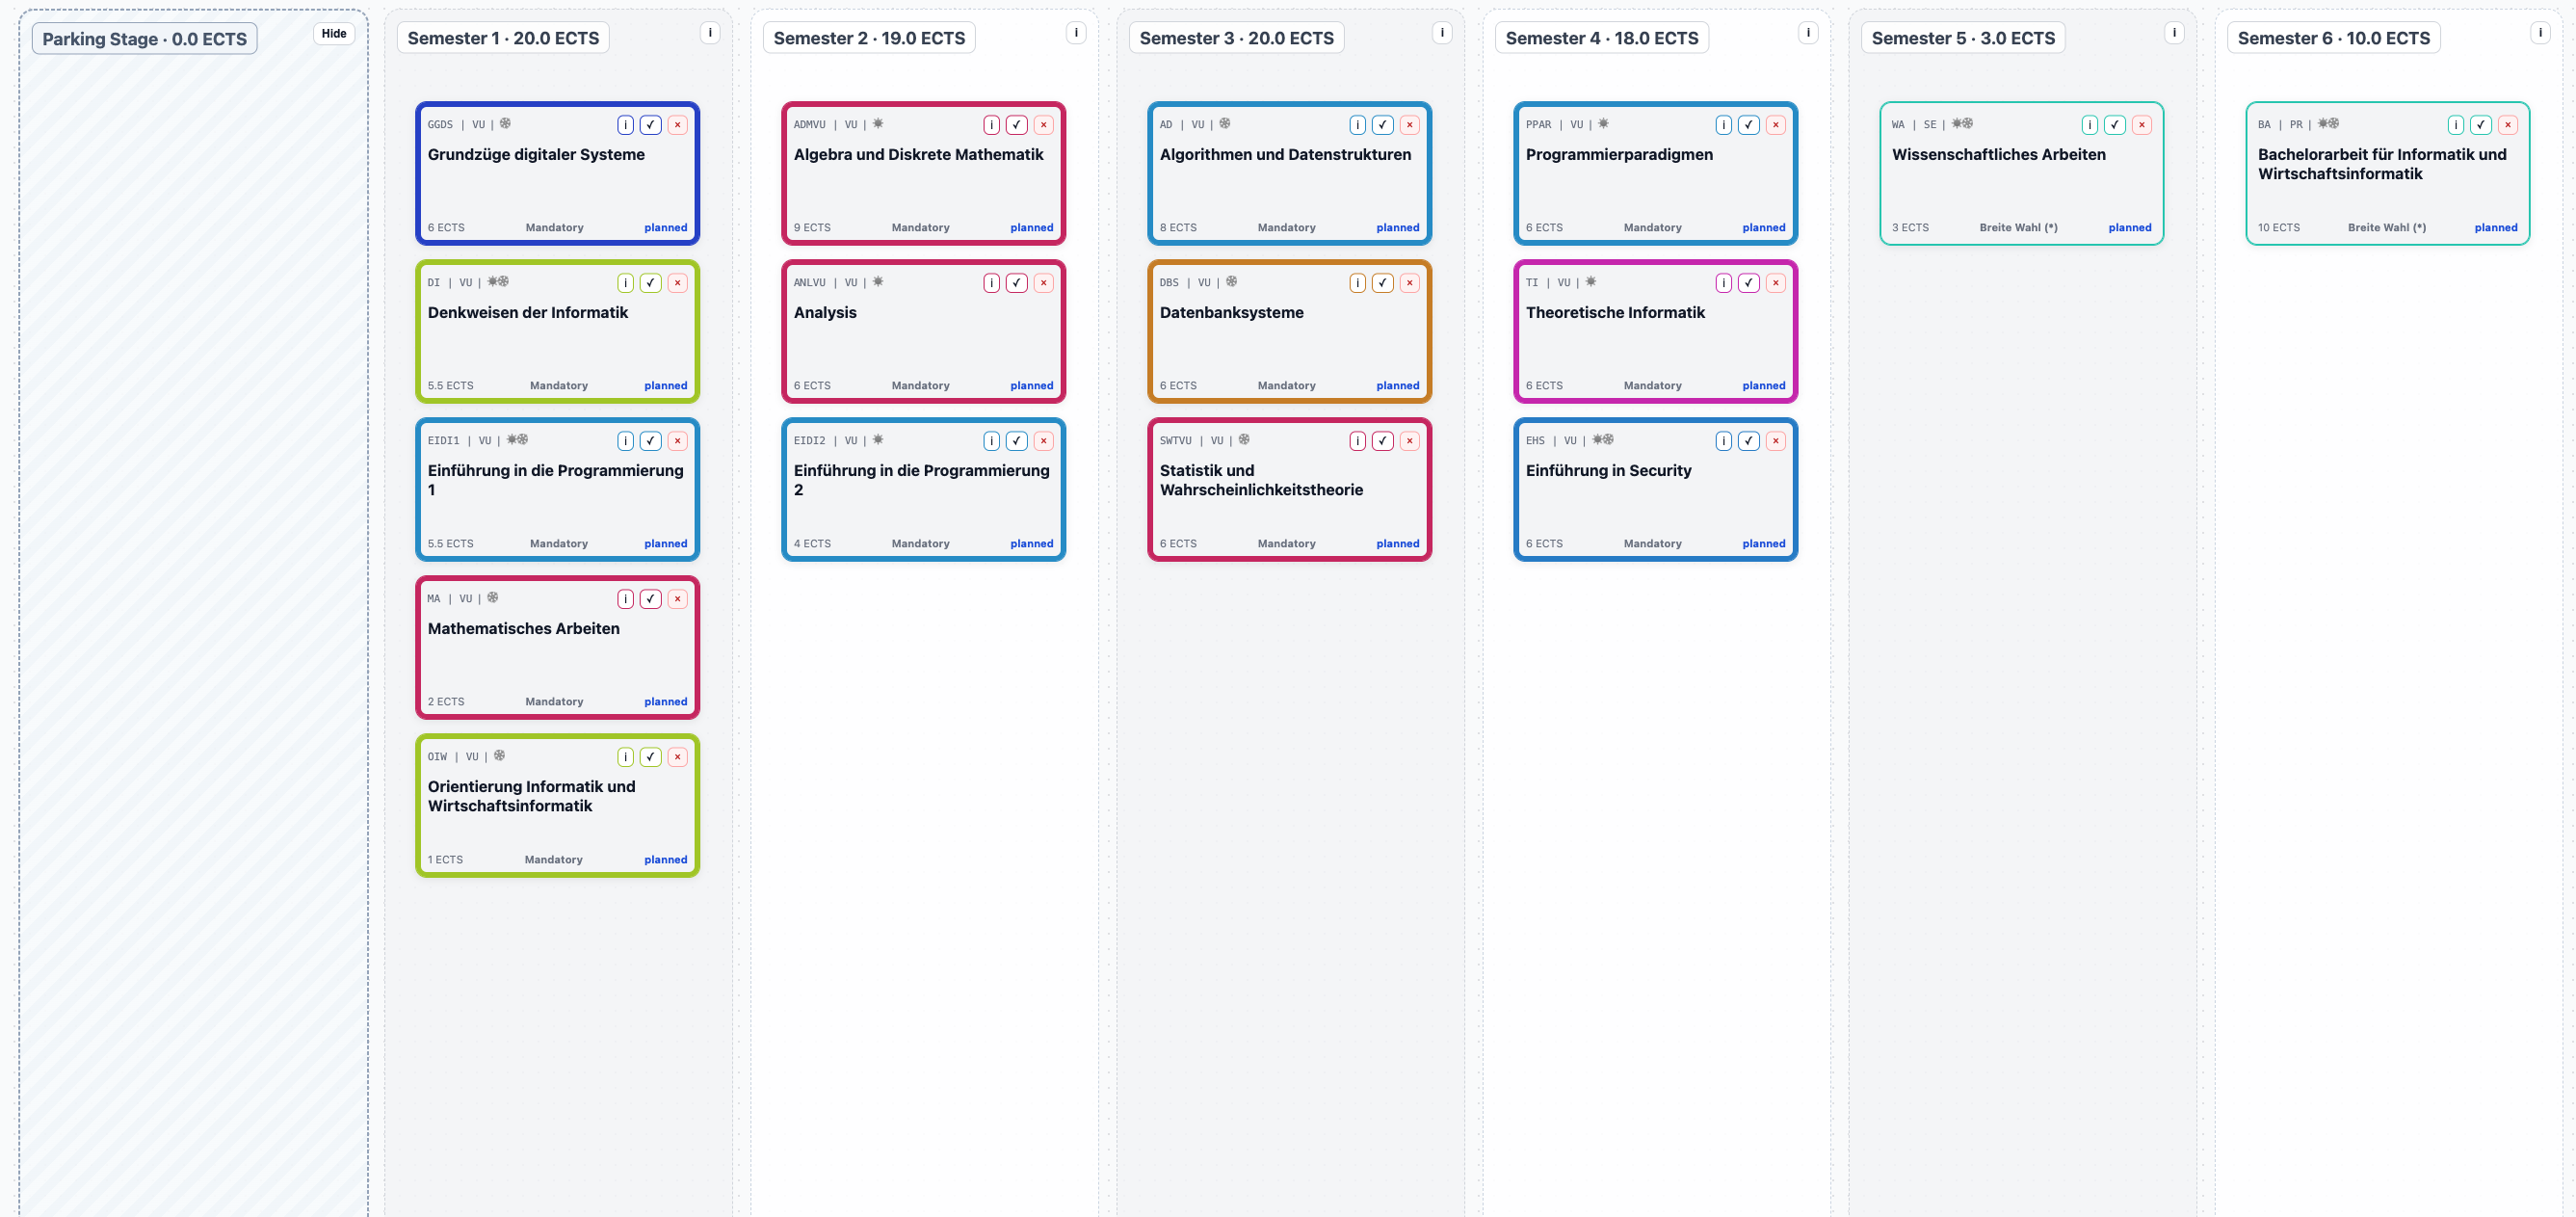
\includegraphics[width=\textwidth]{figures/table_view.png}
\caption{Table View. Semester lanes with running credit totals hold the plan; the Parking Stage on the left holds courses that have been shortlisted but not yet assigned to a semester. Card border colour encodes the exam subject, border weight the obligation type, and the footer carries credits, obligation and status.}
\label{fig:table}
\end{figure*}

\subsection{Graph View}

The Graph View renders the curriculum tree left to right across the four depth levels, with exam subjects stacked as horizontal bands, so that horizontal position encodes depth and vertical band membership encodes the exam subject. Participants had asked for a left-to-right layout ``because we read left to right'' and whether vertical position meant anything; the prototype's radial layout was replaced for both reasons, and a force-directed layout rejected because recomputed positions would destroy spatial memory. Students may drag nodes horizontally within their column and the offset persists; the vertical axis is system-managed. The curriculum's hard prerequisites are drawn as a switchable overlay on the same layout.

A fully expanded Master's programme contains well over 100 nodes, which ``kind of explodes''. Every exam subject and module is individually collapsible, the default is collapsed to the exam-subject level, and a collapsed module is replaced by a placeholder of identical dimensions so nothing reflows. Filtering is a purely visual, reversible layer over six dimensions: obligation type, credit range, course type, exam subject, planning status and term availability; values within a dimension combine disjunctively, dimensions conjunctively.

\subsection{Table View and Parking Stage}

The Table View lays the plan out as one lane per semester, each header showing the semester label and a continuously updated credit total. A course is assigned by dragging it into a lane, or through a Semester Picker anchored to the card that lists only the semesters in which the course is offered, warns where the student's own workload target would be exceeded, and always offers one further future semester so the timeline extends without a configuration step.

Students separate exploring options from committing them to a timeline: finding interesting courses is ``cool as a first step, not thinking yet about which semester''. The tool is therefore built around a three-stage workflow, \emph{browse} (graph or catalogue), \emph{shortlist} (Parking Stage), \emph{assign} (table), with the middle stage optional. The Parking Stage sits directly left of the semester lanes on the same canvas (Figure~\ref{fig:table}), omits chronological and workload indicators, and heads the list in every Semester Picker so that a course found anywhere can be held without a semester decision. A sidebar list was rejected because \emph{parked} is an intermediate state between \emph{not planned} and \emph{planned}, and its position should reflect that progression.

\subsection{Compliance Engine and Dashboard}

Manual rule checking was described as effortful and unreliable (``Excel doesn't know your requirements''). A single compliance check runs after every planning action and reports the plan's status, its hard violations and its soft warnings. Hard violations (a broken hard prerequisite, a semester above the credit ceiling) revert the action and appear as persistent notices; soft warnings (an under-loaded semester, a suboptimal elective sequence) are dismissible advisories, following the requirements-versus-recommendations distinction of \citet{judel_supporting_2023}. Messages name the course, semester and action that triggered them. Regulations are encoded as data, one rule set per programme.

The Dashboard aggregates progress at the four granularities students named, programme, category, semester and module, in collapsible and reorderable sections, with two modes separating what is \emph{planned} from what is \emph{done}. Its programme level carries the checklist of missing requirements. Because every action recomputes it, dropping a course on the canvas already simulates ``what happens if I add this''. Per-semester load is checked against two values held in a personal profile, a recommended target and a maximum, defaulting to 30 and 42 credits; the target is advice, the maximum a limit. The tool never re-balances a plan on the student's behalf.

\begin{figure*}[t]
\centering
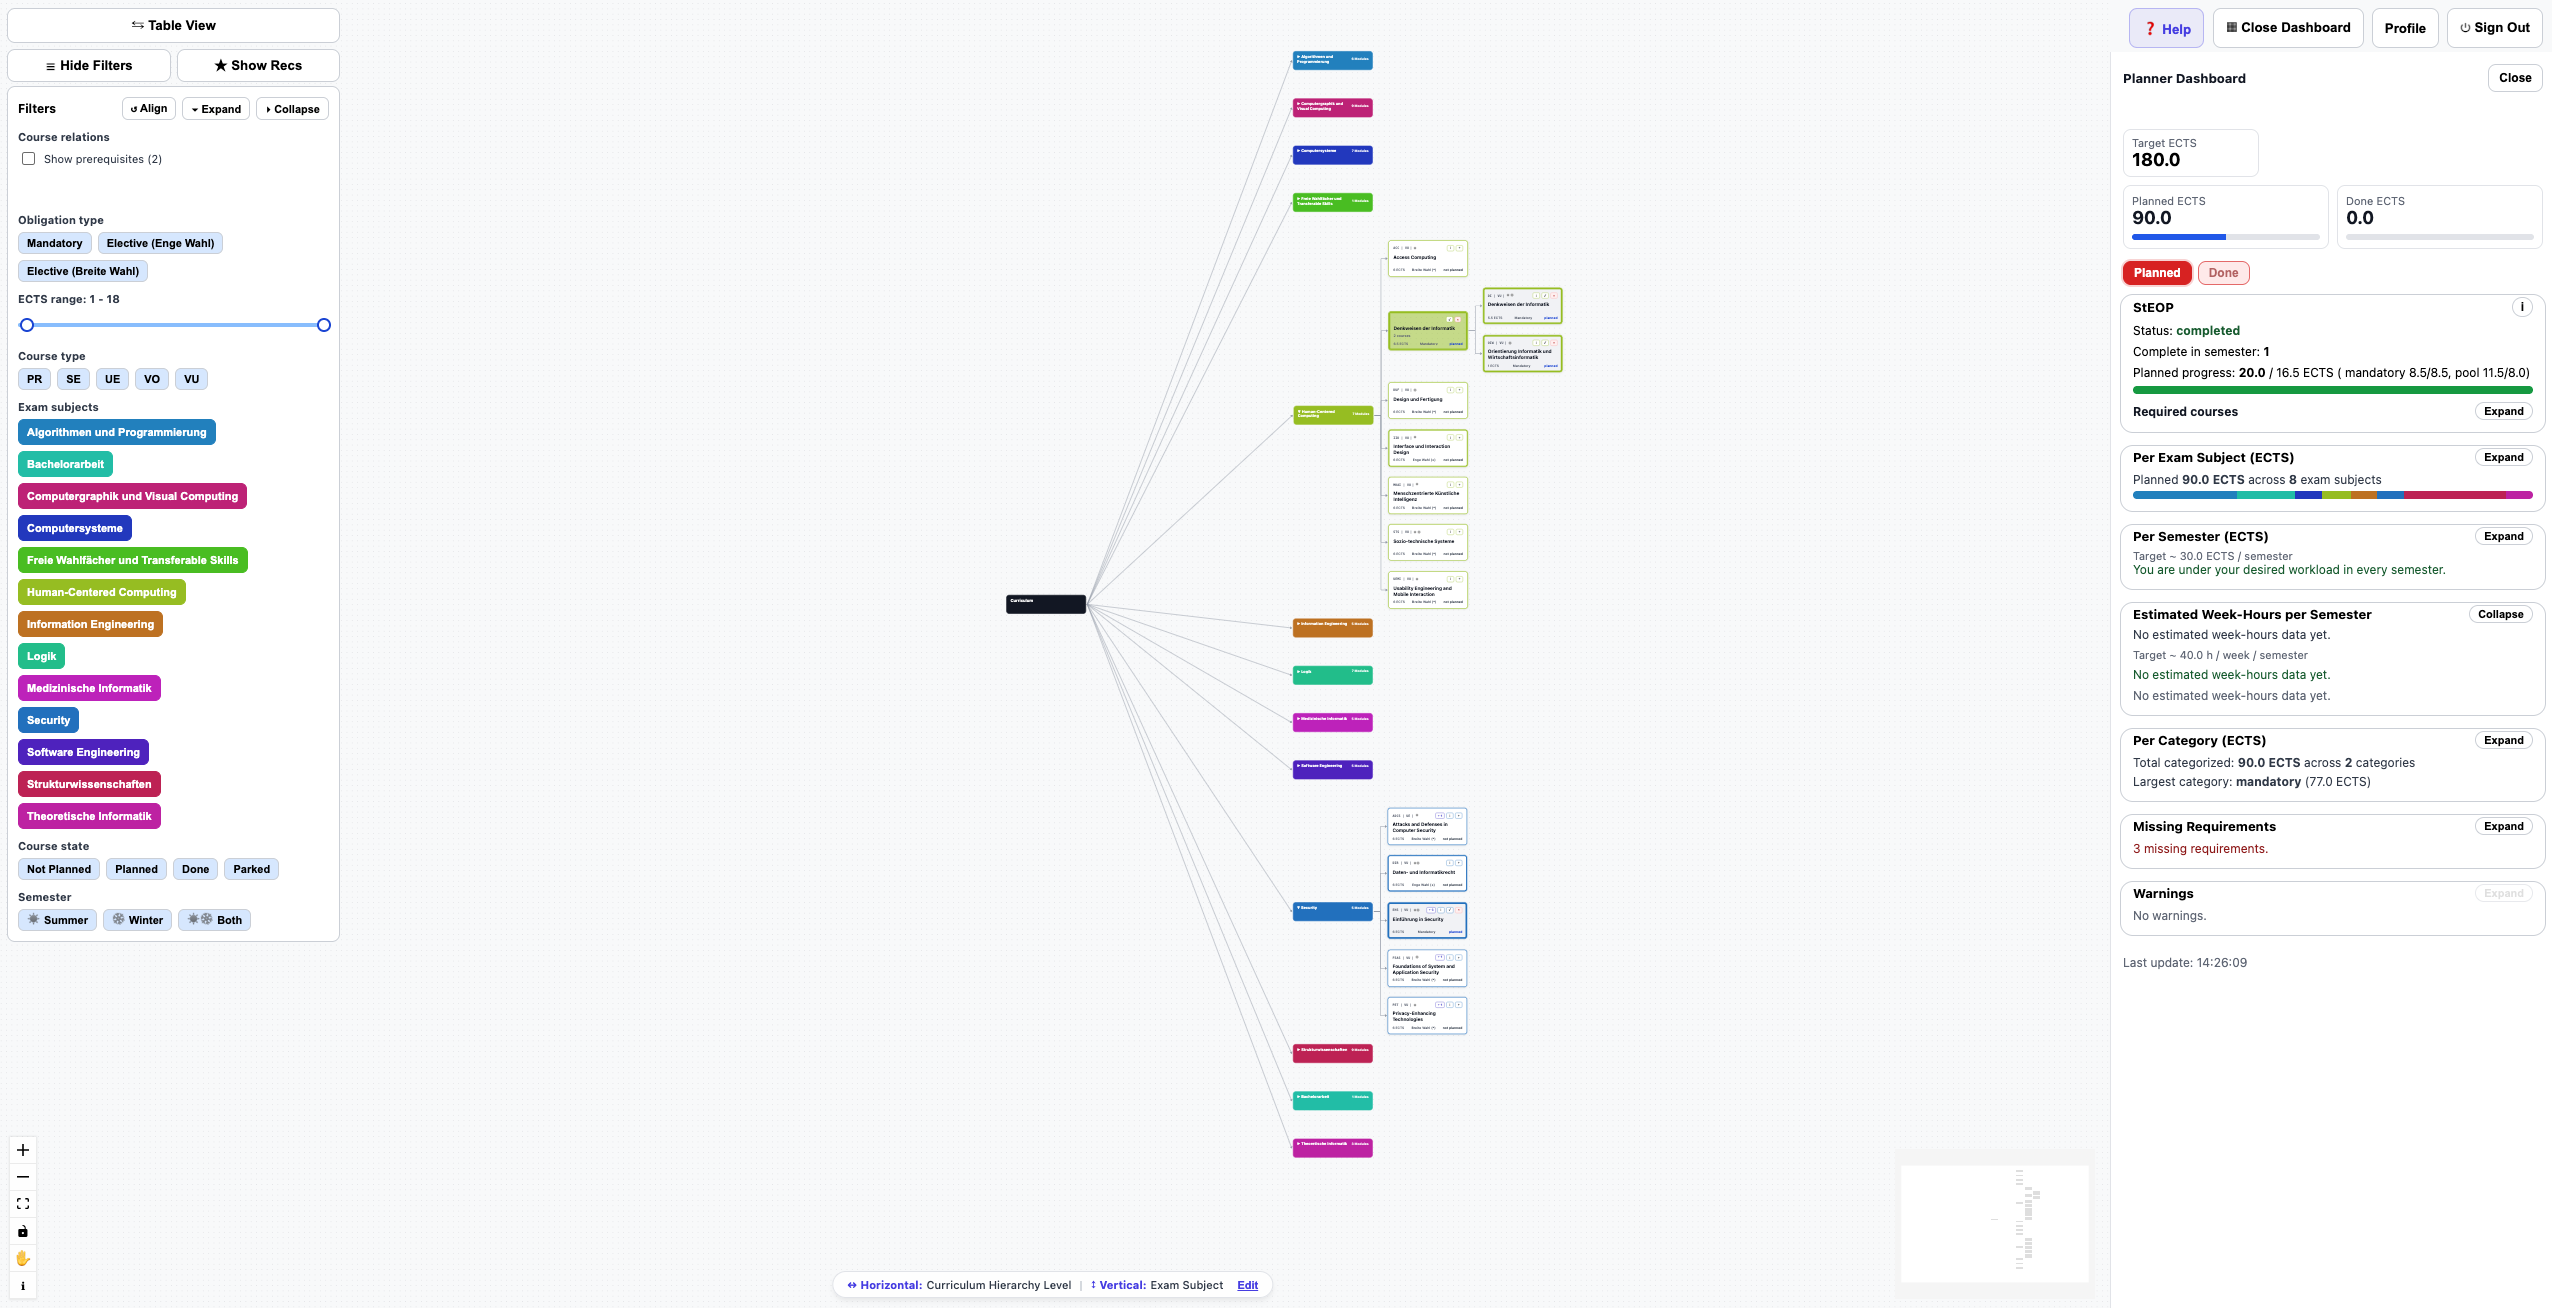
\includegraphics[width=\textwidth]{figures/shell_graph_view.png}
\caption{The three-panel shell with the Graph View active: filter controls on the left, the curriculum tree in the centre drawn left to right from programme to exam subject to module to course with two subjects expanded, and the Dashboard on the right reporting credits, per-subject and per-semester progress, missing requirements and warnings.}
\label{fig:shell}
\end{figure*}

\subsection{Recommendations}

Participants were sceptical of recommendations ``based on nothing'', so the design follows the finding of \citet{ma_courseq_2021} that inspectable explanations raise trust with the algorithm held constant. Rather than a blended score, recommendations come from six named \emph{families}, each of which states its reason on the card in the student's terms: interest match (``matches your interest in machine learning''), curated content similarity, sequence or dependency, internship relevance to a stated career direction, follow-on from a completed course, and peer choice, the last two computed over a cohort of prior plans. Where a signal is weak, the card says so. Recommendations are confined to an independent left-hand panel adjacent to the catalogue; nothing is added to the canvas, and accepting a card uses the same two paths as any course. Recommendation quality is explicitly not a contribution: the behavioural families run on a synthetic cohort, and the engine exists to exercise the workflow of explainable suggestions.

\subsection{Implementation}

The tool is a single-page web client (React, both views on one React Flow canvas) backed by a stateless Python service (FastAPI) and a PostgreSQL database. The recommender scores candidates through six channels behind one protocol, passes the top 100 to the Compliance Engine for trial placement, discards any that would introduce a new error or warning, and returns at most 15. Every state change is timestamped. Six defects observed in the study were closed afterwards, with regression tests; none of those changes was in front of a participant.

% ===========================================================================
\section{\uppercase{Evaluation Study}}
\label{sec:study}

\noindent The study (RQ3) asks how a curriculum graph alters the planning process of students equipped with an established tabular workflow; neither the premise that the graph is useful nor the intended division of labour had been tested. We ran a within-subjects observational study ($N=11$) in which each participant completed comparable planning tasks first with the tabular baseline alone, then with the graph enabled. The design prioritises observational fidelity over outcome comparison: frame-level logging paired with think-aloud transcripts lets the graph's contribution be traced within the process. The fixed order is deliberate: the study asks how a graph enters a workflow a student has already formed, so the baseline had to be formed first, and counterbalancing would not remove the confound, since where a treatment is differently effective at different levels of practice it leaves treatment effects mixed with treatment-practice interactions \cite{greenwald1976within}. Because graph availability and second-task exposure are collinear, we attribute no change in speed or outcome to the graph and ask only whether it displaces the established workflow.

\subsection{Participants and Procedure}

Twelve sessions were run and eleven analysed; one participant declined screen recording. Participants were students of the same faculty as the formative study, enrolled in one of the two target programmes, from their second to eighth semester; four reported regular prior experience with study-planning tools, one little, six none. Each completed two persona-framed planning tasks in a fixed order: \emph{Scenario~A}, a Cybersecurity persona, with the graph unavailable (everything else fully available), and \emph{Scenario~B}, an Artificial Intelligence persona, with the full tool. Each brief stated only the persona's constraints, a per-semester credit band and one reduced-load internship semester, plus guidance on preferred module types; the curriculum's own hard requirements were deliberately not stated and were encountered only inside the tool, so the Dashboard was the sole channel through which curriculum constraints reached participants. Sessions were screen- and audio-recorded in a fixed sequence (demographics, consent, video tutorial, Scenario~A, post-task questionnaire, Scenario~B, post-task questionnaire, open exploration, final questionnaire, semi-structured interview), with think-aloud throughout and a moderator present to unblock operational questions. Post-task questionnaires held three items on task success, plan satisfaction and difficulty plus six domain-adapted items from the Technology Acceptance Model \cite{davis_perceived_1989}; the final questionnaire was the 26-item User Experience Questionnaire (UEQ) \cite{laugwitz_construction_2008}.

\subsection{Analysis}

Two records were collected per participant and triangulated. Screen recordings were sampled every ten seconds, yielding 2,179 frames across the 22 runs, and each frame was coded against a fixed scheme capturing the active surface, open panels, sidebar contents, per-semester credits, Dashboard state and transient banners. Frame coding was executed by a locally hosted vision-language model under a strict protocol (one independent row per frame, no interpolation); its reliability was checked against the first author's manual coding of three complete runs (183 frames). Fixed-interval sampling was chosen because the quantities reported are durations. The method does not see events shorter than ten seconds and records state rather than intent, so every visual code was read against the transcript. Transcripts and recordings were analysed with a deductive codebook classifying usability problems (E-P), positive findings (E-G) and neutral observations (E-N); each code maps to an ISO~9241-11 dimension \cite{iso9241_11}, and problems carry a severity on Nielsen's five-point scale \cite{nielsen1993}. Frequencies are reported as $n/m$, where $m$ is the number of participants for whom the code could be decided.

From the frame labels we derived a state model of the planning process: a state is the primary surface together with the two panels that can vary beside it. In the Table View the Dashboard and the sidebar can each be open or closed, giving \st{dash+cat} (Dashboard open, catalogue in the sidebar: the checklist-driven working state), \st{cat} (catalogue only: browsing), \st{dash} (Dashboard only: reading status) and \st{table} (neither). In the Graph View the sidebar is always the filter panel, so \st{graph} is a single state; \st{off} covers the study guide and questionnaires. The Recommendation Panel stands open across any surface without changing where the student is working, so it is counted as an overlay rather than a state.

% ===========================================================================
\section{\uppercase{Findings}}
\label{sec:findings}

\subsection{The Planning Loop}

Planning under this tool is a single checklist-driven loop with the same shape for every participant: read what the Dashboard says is still missing, find a candidate that closes the gap, place it, and return to the list. The missing-requirements checklist drove task completion for all eleven participants (E-G15, 11/11), and all seeded their plans with the pre-filled mandatory backbone (E-G01, 11/11). P09 opened Scenario~A by reading the count aloud, ``22 missing requirements, wow, that is a lot'', and resolved them item by item. For the most junior participant the loop only emerged after the moderator pointed to the tracker (``exactly that, here I see what I need'').

The loop alternates between the checklist-reading state \st{dash+cat} and a candidate-finding state, which in Scenario~A is the catalogue (Table~\ref{tab:occupancy}). We name its three stages \emph{drive} (reading the checklist), \emph{find} (turning a gap into candidates) and \emph{commit} (placing a candidate). The transition \st{cat}$\rightarrow$\st{dash+cat} accounts for 27.5\,\% of all state changes in Scenario~A and the reverse for 17.4\,\%, so this single pair makes up 44.9\,\% of all logged transitions. The cycle is tight: the median path from an open Dashboard back to the Dashboard is 2.0 transitions ($n=38$ returns), the shortest possible round trip.

\begin{table}[t]
\caption{State occupancy, entries and mean dwell per entry over the eleven runs of each condition (1,197 frames in Scenario~A, 982 in Scenario~B). The catalogue and the graph exchange places. $^{*}$The Recommendation Panel is an overlay counted independently of the states.}
\label{tab:occupancy}
\centering
\footnotesize
\setlength{\tabcolsep}{2.2pt}
\begin{tabular}{@{}lrrrrrr@{}}
\toprule
& \multicolumn{3}{c}{Scenario A} & \multicolumn{3}{c}{Scenario B} \\
\cmidrule(r){2-4}\cmidrule(l){5-7}
State & Occ.\,\% & Entr. & Dwell\,s & Occ.\,\% & Entr. & Dwell\,s \\
\midrule
\st{dash+cat} & 51.2 & 38 & 161 & 46.5 & 51 & 90 \\
\st{cat}      & 27.1 & 40 &  81 &  6.7 & 22 & 30 \\
\st{graph}    & --   & -- &  -- & 26.6 & 42 & 62 \\
\st{dash}     &  5.5 & 11 &  60 &  8.2 &  8 & 101 \\
\st{table}    &  0.6 &  5 &  14 &  2.0 &  3 & 67 \\
\st{off}      & 15.6 & 26 &  72 &  9.9 & 35 & 28 \\
\midrule
\st{recs}$^{*}$ & 24 & 23 & 125 & 20 & 8 & 244 \\
\bottomrule
\end{tabular}
\end{table}

\subsection{What the Graph Changes}

The graph alters the loop at exactly one point: it replaces the catalogue as the surface on which a missing requirement becomes candidate courses, and leaves everything downstream unchanged (Figure~\ref{fig:loop}). In Scenario~B the cycle alternates between the Dashboard and the graph; \st{dash+cat}$\rightarrow$\st{graph} and its reverse each account for 19.3\,\% of state changes (38.6\,\% combined), against the 44.9\,\% the catalogue-Dashboard cycle held in Scenario~A. Occupancy shows the same substitution: catalogue-only occupancy drops from 27.1\,\% to 6.7\,\% while graph occupancy rises to 26.6\,\%, close to the share the catalogue vacates; the catalogue was entered 40 times across the Scenario~A runs and the graph 42 times in Scenario~B, at comparable dwell. The catalogue survives only as a side branch out of the graph. At the participant level, catalogue occupancy falls in ten of eleven cases, from a median of 27.4\,\% to 4.5\,\%. The cycle keeps its shape and period: the median return path to the Dashboard remains two transitions in both conditions. Two things separate this from a practice effect: the graph was made available rather than prescribed, and the catalogue remained available and unchanged. Growing familiarity accounts for a faster second run, not for the abandonment of a surface used competently in the first.

\begin{figure}[t]
\centering
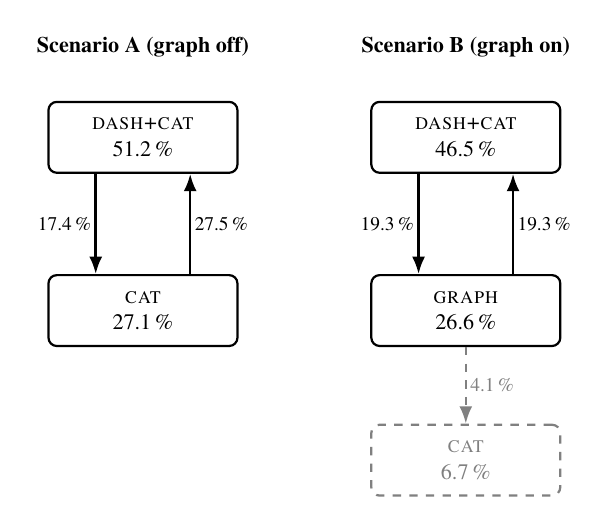
\begin{tikzpicture}[font=\footnotesize,
  s/.style={draw, line width=0.8pt, rounded corners=3pt, fill=white, align=center,
            inner sep=1.5mm, text width=2.1cm, minimum height=9mm},
  faint/.style={s, dashed, draw=gray, text=gray},
  a/.style={-{Latex[length=2.2mm]}, line width=0.9pt, draw=black},
  lb/.style={font=\scriptsize, inner sep=1.2pt, fill=white}]
  \node[font=\footnotesize\bfseries] at (0,1.15) {Scenario A (graph off)};
  \node[s] (dashA) at (0,0)    {\st{dash+cat} \\ 51.2\,\%};
  \node[s] (catA)  at (0,-2.2) {\st{cat} \\ 27.1\,\%};
  \draw[a] ([xshift=-0.6cm]dashA.south) -- node[lb, left]  {17.4\,\%} ([xshift=-0.6cm]catA.north);
  \draw[a] ([xshift= 0.6cm]catA.north)  -- node[lb, right] {27.5\,\%} ([xshift= 0.6cm]dashA.south);
  \node[font=\footnotesize\bfseries] at (4.1,1.15) {Scenario B (graph on)};
  \node[s] (dashB) at (4.1,0)    {\st{dash+cat} \\ 46.5\,\%};
  \node[s] (grB)   at (4.1,-2.2) {\st{graph} \\ 26.6\,\%};
  \draw[a] ([xshift=-0.6cm]dashB.south) -- node[lb, left]  {19.3\,\%} ([xshift=-0.6cm]grB.north);
  \draw[a] ([xshift= 0.6cm]grB.north)   -- node[lb, right] {19.3\,\%} ([xshift= 0.6cm]dashB.south);
  \node[faint] (catB) at (4.1,-4.1) {\st{cat} \\ 6.7\,\%};
  \draw[a, draw=gray, dashed] (grB.south) -- node[lb, right, text=gray] {4.1\,\%} (catB.north);
\end{tikzpicture}
\caption{The dominant planning cycle in each condition, with each transition's share of all state changes and each state's occupancy. Shape and period are unchanged; only the candidate-finding surface differs.}
\label{fig:loop}
\end{figure}

\paragraph{Query Support Without Commit Support.}
The graph supports the \emph{find} step but structurally inhibits the \emph{commit} step. P02 read a missing requirement from the Dashboard, switched to the graph, applied the narrow-elective filter, harvested candidates into the Parking Stage, and returned to the table to place them. Others combined filters for queries the catalogue cannot express, such as term availability with ``not planned''. Conversely, commitment forced a return to the table because the graph renders no semester dimension, so placing a course from a graph node relies on working memory. P10: ``adding directly from here I would probably not do, because I do not know which semester has room''. P06 blindly pushed a semester past its credit cap from the graph, a breach discovered only on returning to the table.

\paragraph{What Does Not Change, and What Cannot Be Attributed.}
Placement accuracy remained stable: the share of placement attempts ending in a system rejection moved from a median of 16.7\,\% in Scenario~A to 13.6\,\% in Scenario~B, decreasing for seven participants and increasing for four, a split consistent with chance (sign test, $p=0.55$). The graph changed \emph{where} candidates were found and left \emph{how} they were committed untouched. The remaining differences are documented but left unattributed because of the fixed order: placements per ten minutes rose from a median of 7.8 to 13.9 (in ten of eleven participants) and sampled time in the planner fell from 20.8 to 13.3 minutes despite a longer second task; six of eleven Scenario~A runs and seven of eleven Scenario~B runs met every constraint of their brief.

\subsection{Around the Loop: Staging, Recommending, Configuring}

\paragraph{The Parking Stage.}
The Parking Stage is what lets two surfaces work on one plan without either doing the other's work, and every participant used it to shortlist before committing (E-G06, 11/11). P04 announced the strategy, ``I will put everything into the parking zone and then go back to the table and assign each to the right semester'', and the recordings show it executed: P09 moved nine courses from graph nodes into the stage in a single episode. That the stage sits outside the plan's accounting is both its function and a source of error: parked credits are excluded from the planned total and nothing on screen says so (E-P38, 10/11). P02 planned against 102 credits while 24 sat parked; two others ended a run with credits parked while the Dashboard reported a complete plan. Nine participants asked for the stage to be visible from inside the graph, where it is not (E-P37, 9/11).

\paragraph{The Recommendation Panel.}
The panel was one of the most occupied surfaces, open for 24\,\% of frames in Scenario~A and 20\,\% in Scenario~B, yet it never entered the cycle. Active stations show frequent entries and short dwells; the panel shows the opposite, 23 entries at a 125\,s mean dwell in Scenario~A and eight at 244\,s in Scenario~B, with 71\,\% of its open time in nine episodes over three minutes. Use divided by how far a student could judge the curriculum alone: ten participants incorporated recommendations (E-G02, 10/11), but seven ultimately bypassed the panel for the checklist and catalogue search (E-N05, 7/11), six of them after having used it successfully earlier, a deliberate choice rather than a discovery failure, while the two participants lacking the knowledge to judge modules independently leaned on the panel and the Dashboard as compensation (E-N06, 2/11). Three defects contextualise this: the overlay occluded the lanes it was meant to populate (E-P11, 6/11); the internships family rendered a bare empty state when the profile's career field was blank (E-P42, 4/11); and four of nine participants could not tell which profile input had triggered a suggestion, although every card gave a reason (E-P68, 4/9).

\paragraph{User-Configured Thresholds.}
Per-semester load is the one rule checked against profile values rather than curriculum data. Aligning them to the brief was part of the task, but a profile left untouched is checked against the defaults with nothing on screen to say so. P01 changed them within four minutes and discovered the asymmetry in the same breath (``I will set it to 33 straight away, more is not allowed, and is there a minimum? No''); P06 completed Scenario~B with a semester at 30 credits against a stated band of 21 to 27 while the Dashboard reported no warning, because the recommended value was still 30 (E-P32, E-P57, 11/11). Students trusted the verdict in both cases.

\subsection{What Worked and Where the Loop Breaks}

Five positive findings are universal: the pre-filled plan removes the blank page, the checklist drives completion, the Parking Stage holds candidates, real-time compliance feedback is noticed and used (E-G04, 11/11), and the graph's filters are valued once found (E-G07, 11/11); nine of eleven used the graph for interest-driven browsing (E-G10) and six said it clarified module composition (E-G17). The most costly problems cluster at the three stages of the loop. At the \emph{drive} stage, status was not glanceable: requirement and credit-gap status lived behind collapsible panels (E-P10, 11/11) and was stated in prose rather than as a figure (E-P03, 7/11), and across the four most recent sessions the warnings panel was never opened while its counter climbed to between two and five. At the \emph{find} stage the catalogue could not be narrowed, since filtering by category, obligation or credits existed only in the graph's sidebar (E-P04, 11/11), so students in Scenario~A fell back on free-text search. At the \emph{commit} stage the lanes did not show whether a semester was winter or summer, so students guessed the term and rejections and rework followed (E-P29, 11/11), the most frequently coded friction: a visualisation deficit rather than a validation error, since the rule was evaluated correctly but the information needed to avoid the error was withheld at the point of decision. Further high-severity problems were the workload band not being enforced (E-P26), completion being signalled over an incomplete constraint set (E-P34), the graph carrying no semester dimension (E-P47, 10/10), and unclear curriculum terminology (E-P01, 4/11).

\subsection{Questionnaires}

The UEQ describes a tool judged capable before engaging: pragmatic quality $+2.28$ outscores hedonic quality $+2.00$ on the $-3$ to $+3$ scale, attractiveness ($+2.61$) and efficiency ($+2.59$) lead, and the two weakest scales map onto the qualitative record. Perspicuity ($+1.82$, SD~0.70) reflects the learnability and terminology friction above; novelty ($+1.77$, SD~0.78) reflects that participants read the tool as a better version of what they already did (P04: ``until now I only edited Excel files manually, I find this really great''). The adapted TAM items rate high in both conditions (ease of use 5.59 and 6.09 of 7; usefulness items 6.09--6.64), read descriptively given the fixed order. The instructive result is a single item: satisfaction with the finished plan is the only rating that falls, from 6.27 to 5.91, and the two largest drops belong to the participants whose Scenario~B plans went furthest wrong, whereas on the same sheet the success item rated seven of the eight failed runs successful. Students' judgement of the plan tracked its measured quality; their judgement of their own success did not.

\subsection{The Plans Produced, Against Self-Report}

Every finished plan was audited against its brief. Of 21 resolved runs, 13 met every constraint. Of the eight failures, four missed the reduced-load internship semester, two fell short of the degree total, and two exceeded the maximum workload through the profile mismatch above. Participants rated seven of the eight failed runs as successful, so self-reported success tracked \emph{felt} rather than actual completion (E-N03, 9/11). In all 22 runs the Dashboard ultimately reported zero missing requirements, correctly against the curriculum's rules and silently against the task's. P02 correctly reserved an empty lane for the internship; because the system has no way to register an internship semester, the Dashboard flagged a missing credit total, and P02, trusting the interface over the brief, filled the lane to clear the warning. An unrepresented constraint is not merely left unverified; it actively competes with the constraints the checklist does display, and the interface won in every case observed.

% ===========================================================================
\section{\uppercase{Discussion}}
\label{sec:discussion}

\noindent The design rested on several untested assumptions; the evaluation speaks to each. The result is a \emph{process, not a feature}: one loop in which the pre-fill seeds a plan, the checklist drives it, catalogue, graph and recommendations propose candidates, the Parking Stage holds them and the table commits them, externalising exactly the part of programme planning students cannot hold in their heads. \emph{The Dashboard as compass} did more than intended: because the briefs stated no curriculum rules, participants met the curriculum only through it, so it did not support an understanding of the curriculum, it constituted one, and what it did not hold them to did not exist for them. \emph{A staging area between finding and committing} mattered more than the design claimed: a shared-plan hybrid does not need each view to do everything, but it needs an explicit place for a decision made and not yet committed. \emph{Graph for exploration, table for commitment} held with a narrower scope and for a different reason: graph activity was directed querying, the division was driven by missing context (no lanes, no totals) rather than by representational limits, and the query step's value came largely from the filter panel, which leaves open how much would survive if the table shared those filters. \emph{Drawing only what the curriculum fixes} was sound as a rule and empty in application: the Bachelor's programme fixes no ordering between two named courses, so the overlay was empty rather than sparse, and four participants asked for ordering at the point of placement. \emph{Guide rather than block} was supported, but the tiering was asymmetrical, a hard block above the ceiling and a dismissible warning below the floor, assigned by how a breach sounds rather than what it costs, and the thresholds came from a profile whose defaults silently validated plans against the wrong values. \emph{Recommendations with reasons} held for use and half held for reasons: they served the least expert users most, while confident users wanted a different route to the same end.

\subsection{Design Implications}

Six rules follow for interfaces that guide a user through a constrained, multi-step decision, of which a study planner is one instance.
\begin{itemize}
  \item \textbf{An authoritative signal must cover every actual constraint.} Users do not read a partial completion signal as partial. Pending work should be counted or visibly excluded, and active defaults announced.
  \item \textbf{Tier rules by the cost of the breach}, not by how it sounds; opposing bounds of one constraint should carry the same friction.
  \item \textbf{Allow commitment only from views that show the consequences.} A view that cannot show what an action alters should be restricted to finding and staging.
  \item \textbf{Put decision-making data where the decision happens.} Filters lived in the graph while placement happened in the table; status lived behind collapsed panels.
  \item \textbf{Show valid targets before an action is attempted}, rather than rejecting invalid attempts afterwards.
  \item \textbf{Treat guided and self-directed workflows as equals}, and make automated guidance explain its inputs so confident users can audit rather than discard it.
\end{itemize}

\subsection{Relation to Prior Work}

The findings are \emph{consistent with} the friction points \citet{bartel_design_2024} report for study-planning assistants: reading institutional terminology and finding nested filters. They \emph{qualify} the premise of the graph-visualisation literature \cite{zucker_vicurrias_2009,auvinen_stops_2014,trippel_developing_2025} that a curriculum carries a prerequisite network worth drawing: the curricula studied here carry little of one, the graph draws containment rather than sequence, and a prerequisite advisory arose once in 22 runs. They \emph{extend} the AIStudyBuddy lineage \cite{roepke_study_2024,judel_supporting_2023,trippel_developing_2025} by observing the process of forming a plan rather than its reception or its post-hoc paths: positive reception is reproduced, but it does not predict the graph's role, which was a query surface that displaced the catalogue.

The completion finding gives the dashboard critique a counterpart at the level of the individual student. \citet{caulfield2013} objected that Course Signals was credited beyond what had been checked; here the Dashboard reported no missing requirements, correctly for the curriculum and silently for the task, and participants read that report as completion in preference to their own model. \citet{parasuraman1997humans} describe the hazard as misuse of automation, over-reliance governed among other things by the saliency of a system's state indicators; a completion checklist is exactly such an automation, continuous, salient and silent about what it has not checked. The split in recommendation use speaks to the integration called for by \citet{bodily_review_2017}: the components were available together but not used as a whole, with a division of labour dictated by curriculum confidence, the same line \citet{ma_courseq_2021} found between students with and without clear goals. Finally, the displacement of the catalogue by the graph is an instance of cognitive fit \cite{vessey1991cognitive}: spatial tasks are served by graphs, symbolic tasks by tables, and the hybrid makes that distinction physical.

\subsection{Limitations}

The requirements come from six students at one faculty, elicited around a prototype that already assumed a graph-and-table interface, so the formative study shaped how such an interface should behave without testing whether students want one. The fixed task order entangles the graph's introduction with practice effects, which is why only displacement and rejection share are interpreted. Eleven computing students at one institution, likely more comfortable with node-link diagrams than the general student body, bound generalisation, and any pattern by expertise rests on very small subsets. The first author designed the tool, moderated the sessions and coded the results, so the near-ceiling questionnaire scores are vulnerable to demand characteristics, which is why the screen recordings are treated as the stronger evidence; participants planned for a fictional persona under a time limit. Frame sampling at ten seconds misses shorter events and intent, and frames were coded by a vision-language model checked against manual coding of three runs.

% ===========================================================================
\section{\uppercase{Conclusion}}
\label{sec:conclusion}

\noindent We designed, built and evaluated a hybrid graph-table interface for programme-level study planning and observed how students use it. RQ1 is answered by a specification of 13 features and 55 requirements traceable to interview evidence. RQ2 is answered by the artefact, whose central decision, a single authoritative plan model from which both views and all feedback derive, is what makes the views projections of one plan rather than two plans to reconcile. RQ3 is answered by a consistent checklist-driven loop in which the graph substitutes for the catalogue at the query step, largely through its filters, and does not support the commit step; by a staging area that proved essential as the hinge between the views; by recommendations that were used heavily at first and set aside once students could judge the curriculum themselves; and by an over-reliance on the tool's completion signal that let constraints the checklist did not model fall out of working memory.

The findings generalise in three widths: the completion finding does not depend on study planning at all; the loop, the pre-filled backbone and the split of recommendation use by confidence need only a checklist and a recommender; and the graph at the query step, its dependence on its filters and the Parking Stage as the hinge are specific to hybrids. Each is a hypothesis for a larger study, and one is directly falsifiable: if the graph's value lies in its filter panel, adding those filters to the table should render the graph largely optional. Because the system timestamps every state change, the process account can be scaled into a log study of students planning their actual degrees. Where curricula encode few hard dependencies, future work should reconsider what a curriculum graph ought to display, perhaps broad eligibility gates rather than a sparse prerequisite network, and should test expertise-moderated tool use with a sample drawn from beyond computing programmes.

% ---- Camera-ready only. Removed for double-blind review. ----------------
% \section*{\uppercase{Acknowledgements}}
% \begin{itemize}
%   \item \textbf{Conflicts of Interest:} The authors have no conflicts of interest to declare.
%   \item \textbf{Financial and other Support:} No funding was received for the work reported here.
%   \item \textbf{Data Sharing:} ...
%   \item \textbf{AI Tools:} State here, per the CSEDU policy, which AI tools were used,
%         for which parts of the paper, and how (e.g. condensing the thesis text into
%         this paper, language editing). Cite the AI system in the affected sections.
% \end{itemize}

\bibliographystyle{apalike}
{\small
\bibliography{references}}

\end{document}
